\documentclass[a4paper]{article}
\usepackage{cmap}
\usepackage{mathtext}
\usepackage{amssymb}
\usepackage{amsmath}
\usepackage[russian]{babel}
\usepackage{indentfirst}
\usepackage[pdftex]{graphicx}
\usepackage{multirow}
\usepackage{mathrsfs}
\usepackage{biblatex}
\usepackage{siunitx}
\usepackage[left=2cm,right=2cm,top=2cm,bottom=2cm]{geometry}
\usepackage{fancyhdr}
\bibliography{bib}
\pagestyle{fancy}
\newcommand{\rref}[1]{(\ref{#1})}
\newenvironment{comment}{}{}
\newcommand{\picref}[1]{рис. \ref{#1}}
\newcommand{\mbf}{\mathbf}
\newcommand{\Equip}[3]{
	
	{\bf #1:} $\Delta = \pm #2\; #3$}
\newcommand{\equip}[1]{
	
	{\bf #1}}
\newcommand{\labname}{Интерферометр Фабри---Перо} 	% название пиши здесь
\newcommand{\labnum}{4.4.4}		% номер вводи здесь
\fancyfoot{}
\fancyhead[RE, RO]{\thepage}
\fancyhead[LE, LO]{Лабораторная работа \labnum \space \labname}
\title{Лабораторная работа \labnum \space \labname} % Название работы здесь
\author{Иван Сладков}
\begin{document}
\maketitle
\thispagestyle{empty}
\section{Аннотация}
В данной работе проводится измерение длины волны жёлтых линий ртути, жёлтого дублета натрия, а также определение спектральных характеристик интерферометра Фабри—Перо. 

\section{Теоретические сведения}

Интерферометр Фабри–Перо состоит из двух стеклянных или кварцевых пластин с хорошо отполированными поверхностями. На одну поверхность каждой пластины нанесены отражающие свет покрытия. Интерферометр можно рассматривать как плоскопараллельную пластину, в которой происходят многократные отражения и интерференция световых волн (рис. \ref{fig:reflections}). 

\begin{figure}[]
	\centering
	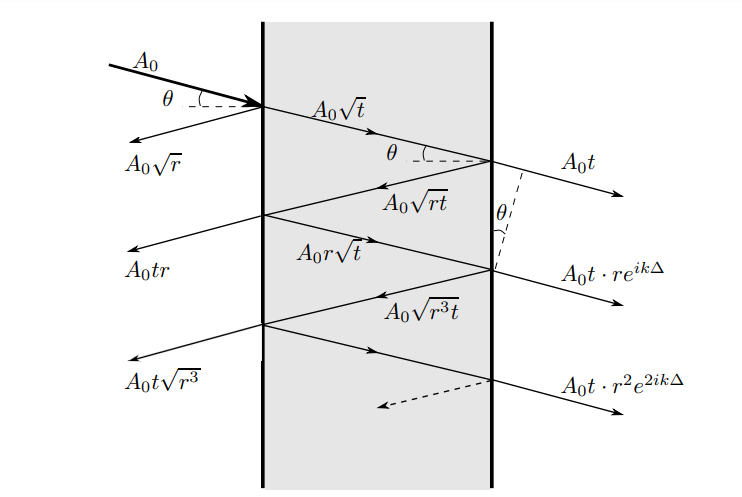
\includegraphics[width=0.8\linewidth]{Screenshot_1}
	\caption{Прохождение волны через интерферометр Фабри---Перо}
	\label{fig:reflections}
\end{figure}

Найдём условие возникновения интерференционной картины для световой волны с длиной $ \lambda $. Выразим разность хода двух интерферирующих волн, падающих на интерферометр под углом $ \theta $:

\begin{equation*}\label{key}
	\delta = 2 L \cos \theta,
\end{equation*}
где через $ \delta $ обозначена разность хода двух волн, а через $ L $ -- база интерферометра. Отсюда условие максимума интенсивности интерферирующих волн:
\begin{equation*}\label{key}
	2 L \cos \theta_m = m \lambda.
\end{equation*}
Оно же является условием резонанса, при выполнении которого интерферометр просветляется для данной длины волны $ \lambda $.

\begin{figure}[]
	\centering
	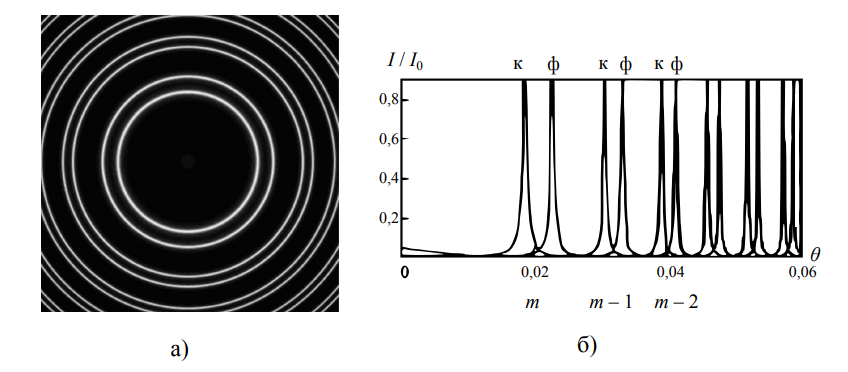
\includegraphics[width=0.8\linewidth]{Screenshot_2}
	\caption{а) Наблюдаемая интерференционная картина; б) Зависимость интенсивности света от угла $ \theta $}
	\label{fig:screenshot2}
\end{figure}

Для малых углов и больших порядков спектра угловая дисперсия определяется соотношением:
\begin{equation*}\label{key}
	D = \frac{d \theta}{d \lambda} = - \frac{m}{2 m \sin \theta_m} \approx - \frac{1}{\lambda \theta_m}.
\end{equation*}

Разрешающая способность для порядка спектра $ m \approx \frac{2 L}{\lambda} $:
\begin{equation*}\label{key}
	R = \frac{\lambda}{\Delta \lambda}= \frac{\pi\sqrt{r} m }{(1-r)}
\end{equation*}

\section{Оборудование и инструментальные погрешности}

Экспериментальная установка, применяемая в данном опыте, схематически изображена на рис. \ref{fig:scheme}. Свет от лампы, пройдя через линзу и светофильтр, попадает на интерферометр Фабри—Перо. Линза $ Л_0 $ служит для формирования пучка лучей (слегка сходящегося или слегка расходящегося). Интерференционные кольца наблюдаются в фокальной плоскости линзы Л через зрительную трубу, сфокусированную на фокальную плоскость. Диаметры колец измеряются с помощью микроскопа катетометра.

\begin{figure}[]
	\centering
	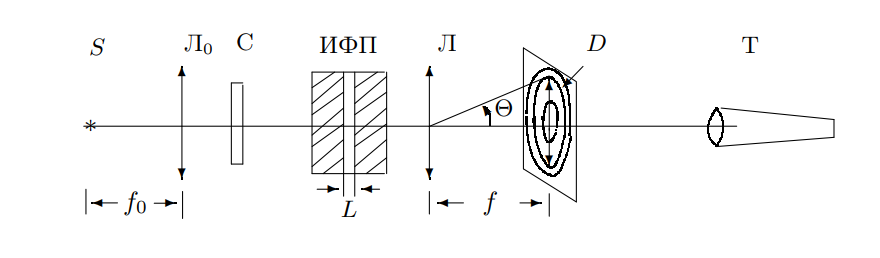
\includegraphics[width=0.8\linewidth]{Screenshot_3}
	\caption{Схема экспериментальной установки}
	\label{fig:scheme}
\end{figure}

\equip{Интерферометр Фабри---Перо}: $ L = 0.1\; мм $
\equip{Линзы}: $ f = 110\; мм $
\equip{Светофильтры}
\equip{Ртутная и натриевая лампы}
\Equip{Катетометр КН-6}{0.001}{мм}

\section{Результаты измерений и обработка данных}
\emph{Все измерения и расчёты в СИ.}

\subsection{Ртутная лампа}

\paragraph{Зелёный светофильтр}

Измерим координаты колец (табл. \ref{tab:greendata}).

\begin{table}[h]
	\centering
	\begin{tabular}{|l|l|l|l|}
		\hline
		$ n $ & $a_{верх} $ & $a_{низ}$ & D     \\ \hline
		1     & 190.42      & 175.51    & 14.91 \\ \hline
		2     & 193.75      & 172.37    & 21.38 \\ \hline
		3     & 196.1       & 169.54    & 26.56 \\ \hline
		4     & 198.08      & 167.77    & 30.31 \\ \hline
		5     & 199.74      & 166.37    & 33.37 \\ \hline
	\end{tabular}
	\caption{Координаты максимумов колец для зелёного светофильтра}
	\label{tab:greendata}
\end{table}

По ней построим график $ D^2(n) $ на рис. \ref{fig:screenshot5}.

\begin{figure}[]
	\centering
	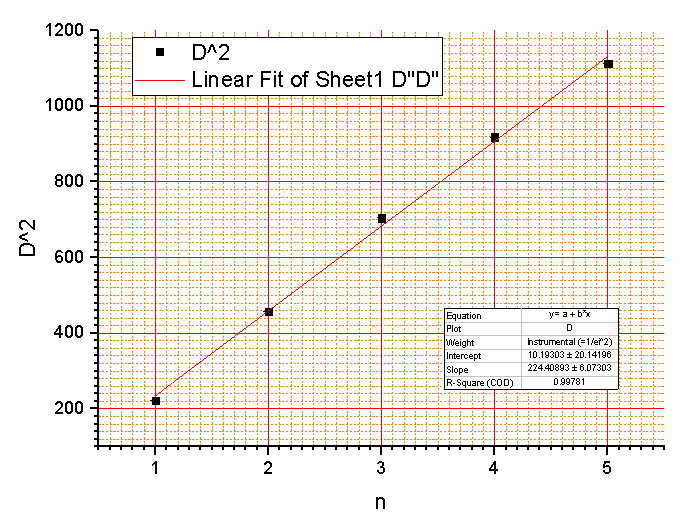
\includegraphics[width=0.8\linewidth]{Screenshot_5}
	\caption{График $D^2(n)$}
	\label{fig:screenshot5}
\end{figure}

По углу наклона $ k = \lambda / L = 224\pm 6 $ найдём базу интерферометра:
\begin{equation*}\label{key}
	L=\frac{4 f^2 \lambda}{k} = 0.12 \pm 0.01\; мм,
\end{equation*}
что неплохо согласуется с фактическим значением.

\paragraph{Жёлтый светофильтр}

Для жёлтого компонента спектра ртути замерили координаты 5 колец. Результаты в табл. \ref{tab:yellowdata}. По этим данным построим график на рис \ref{fig:screenshot4}. Систематическая погрешность значений не более $ 1 \% $ -- пренебрегаем.

\begin{table}[h]
	\centering
	\begin{tabular}{|l|l|l|l|l|l|l|}
		\hline
		$ n $ & $a_{верх}^{тёмн} $ & $a_{низ}^{тёмн}$ & $a_{верх}^{светл} $ & $a_{низ}^{светл} $ & $1/\Delta D$ & $\overline{D}$ \\ \hline
		1 & 189.53 & 178.32 & 186.78 & 180.85 & 0.18939 & 8.57   \\ \hline
		2 & 193.65 & 173.98 & 192.53 & 175.22 & 0.42373 & 18.49  \\ \hline
		3 & 196.61 & 171.27 & 195.64 & 171.99 & 0.59172 & 24.495 \\ \hline
		4 & 198.84 & 168.74 & 198.13 & 169.47 & 0.69444 & 29.38  \\ \hline
		5 & 201.1  & 166.71 & 200.28 & 167.19 & 0.76923 & 33.74  \\ \hline
	\end{tabular}
	\caption{Координаты максимумов колец для <<тёмного>> и <<светлого>> жёлтых светофильтров }
	\label{tab:yellowdata}
\end{table}

\begin{figure}[]
	\centering
	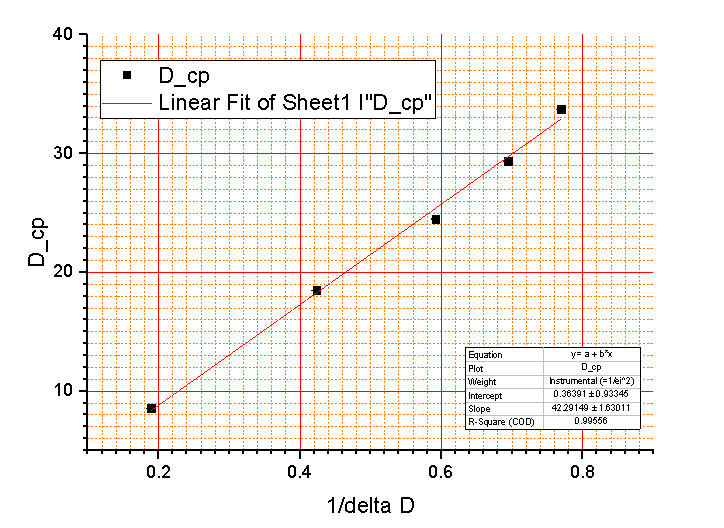
\includegraphics[width=0.8\linewidth]{Screenshot_4}
	\caption{График зависимости $\overline{\Delta D}(\frac{1}{D})$}
	\label{fig:screenshot4}
\end{figure}

Из графика найдём $ \Delta \lambda $ -- разность длин волн жёлтой пары ртути.

\begin{equation*}\label{key}
	\Delta \lambda = \frac{\lambda \overline{D} \Delta D}{4 f^2} = \frac{\lambda k}{4f^2} = (4.9 \pm 0.2) \; \SI{}{\angstrom}
\end{equation*}
Здесь погрешность получена из относительной погрешности $ k $.


Оценим максимальный порядок интерференции $m$ для желтой линии ртути:

\[
m_\text{жёл} = \frac{2L \cos \theta}{\lambda} \approx \frac{2L}{\lambda} = 345
\]

Кроме того, оценим дисперсионную область:

\[ \Delta \lambda_{жёл} = \frac{\lambda^2}{2 L}= 149 \; \SI{}{\angstrom}. \]

Найдём разрешающую способность прибора:
\begin{equation*}\label{key}
	 \delta r = (0.8 \pm 0.01) \;  мм 
\end{equation*}
\[ R = \frac{4f^2}{D \delta r} = 5040 \pm 100 \]
Погрешность определяется по соответствующей формуле для сложения инструментальных погрешностей.

Найдём добротность:
\[ Q = \frac{2 \pi L}{\lambda (1 - r)} = 7600 \pm 300\]
при $ r=0.85 $

Отсюда число интерферирующих лучей: 
\[N = \frac{Q}{m} = 21\]


\subsection{Натриевая лампа}

Аналогично, построим графики $ D^2(n) $ и $ \overline{D}(1/\Delta D) $ на рис. \ref{fig:screenshot6} и рис. \ref{fig:screenshot7} соответственно.

\begin{table}[h]
	\centering
	\begin{tabular}{|l|l|l|l|}
		\hline
		n & $D^2$ & $\overline{D}$ & $1/\Delta D$ \\ \hline
		1 & 80    & 8.96           & 0.50251      \\ \hline
		2 & 299   & 17.299         & 1.02145      \\ \hline
		3 & 519   & 22.776         & 1.35135      \\ \hline
		4 & 725   & 26.925         & 1.47059      \\ \hline
		5 & 938   & 30.6215        & 1.82648      \\ \hline
		6 & 1142  & 33.795         & 1.8018       \\ \hline
	\end{tabular}
	\caption{Данные для построения графиков 6, 7 (Натрий)}
	\label{tab:my-table}
\end{table}

Так же найдём базу интерферометра:
\begin{equation*}\label{key}
	L = 0.13\pm 0.01 \; мм.
\end{equation*}

Найдём разность длин волн:
\begin{equation*}\label{key}
	\Delta \lambda = \frac{\lambda k}{4 f^2} = 5.6\pm 0.3\; \SI{}{\angstrom}
\end{equation*}

Следует заметить, что одна из точек графика \ref{fig:screenshot7} не ложится на прямую -- видимо, дрогнула рука -- поэтому эту точку пришлось не учитывать.

\begin{figure}[]
	\centering
	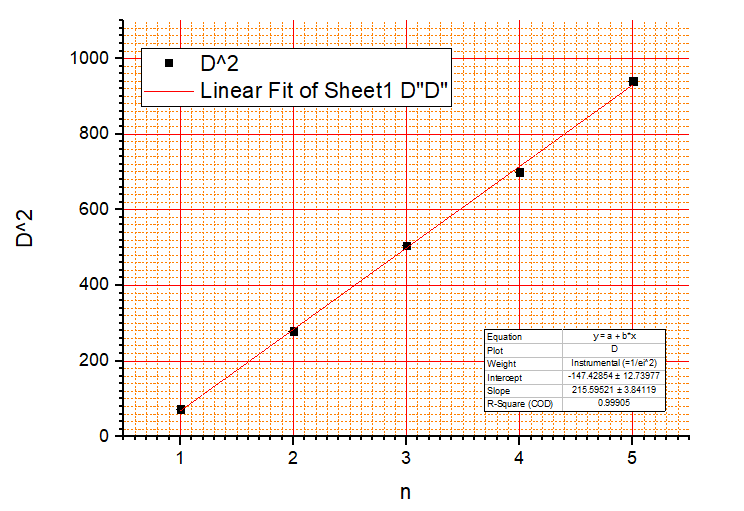
\includegraphics[width=0.8\linewidth]{Screenshot_6}
	\caption{График зависимости $ D^2(n)$}
	\label{fig:screenshot6}
\end{figure}

\begin{figure}[]
	\centering
	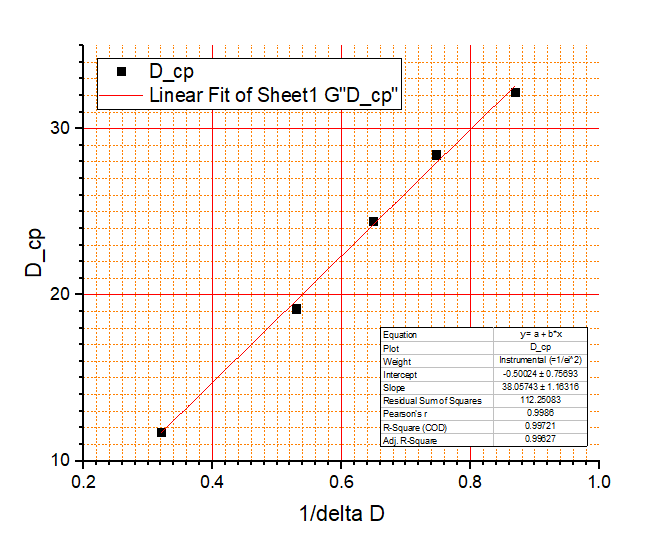
\includegraphics[width=0.8\linewidth]{Screenshot_7}
	\caption{График зависимости $\overline{D}(1/\Delta D)$}
	\label{fig:screenshot7}
\end{figure}

Оценим линейную дисперсию интерферометра для $ n = 5 $ для ртути:

\[ D^*_{эксп} = \frac{\Delta D}{2 \Delta \lambda} = 0.54\pm 0.08 \; мм/\SI{}{\angstrom}; \quad  D^*_{теор} = \frac{2f^2}{\lambda D} = 0.44 \; мм/\SI{}{\angstrom} \]


\section{Вывод}

По результатам проведённых опытов, определили характеристики интерферометра Фабри---Перо, а также исследовали спектры ртути и натрия, в частности длины волн жёлтых линий ртути и жёлтого дублета натрия; определили для них разность длин волн.

\newpage
\begin{thebibliography}{9}
	\bibitem{Siv} Сивухин Д. В. \emph{Общий курс физики. Том 4 Оптика}, 2004
	\bibitem{kir} Кириченко Н. А. \emph{Принципы оптики}, 2014
	\bibitem{max} \emph{Лабораторный практикум по общей физике. В 3 томах. Том 2. Оптика: учебное пособие} под ред. А. В. Максимычева
\end{thebibliography}
\end{document}